\chapter{Технологический раздел}

В технологическом разделе выбраны и описаны средства реализации программного обеспечения и представлены детали его реализации.
В качестве языка программирования был выбран С++,~т.~к. он 
как он позволяет реализовать все алгоритмы, выбранные в результате проектирования, а также поддерживает все требуемые структуры данных. Для создания пользовательского интерфейса использовался фреймворк Qt,~т.~к. в нем присутствуют необходимые для этого инструменты, для задач визуализации --- библиотека SFML.

\section{Графический интерфейс программы}
На рисунке~\ref{fig:interface} представлен интерфейс программы. Интерфейс позволяет загрузить модель вулкана, задать скорость и направление ветра, частоту вывода кадров симуляции и перейти к окну визуализации. 

\begin{figure}[H]
	\centering
	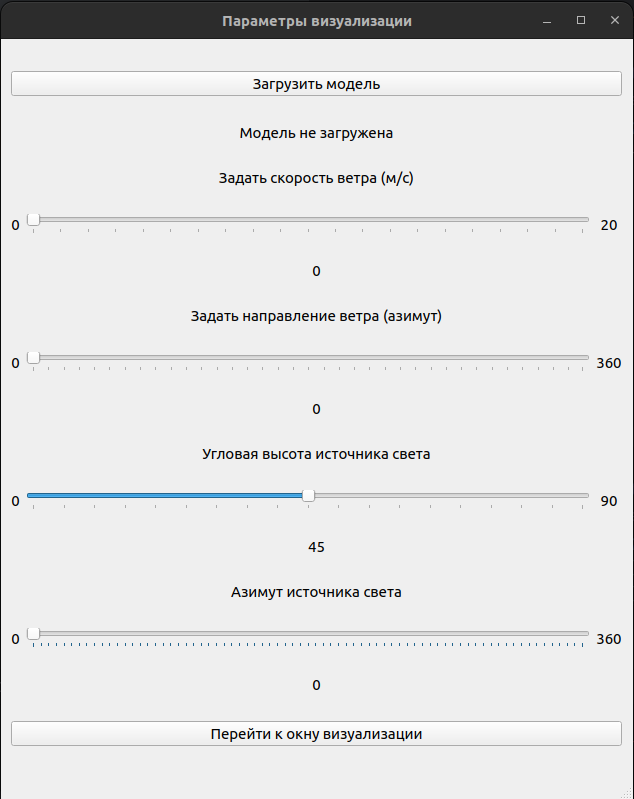
\includegraphics[width=1.0\textwidth, page=1]{assets/img/interface.png}   
	\caption{Интерфейс программы.}
	\label{fig:interface}
\end{figure}
\section{Реализация алгоритмов}

В листинге~\ref{lst:z_buf} представлен листинг функции с использованием z-буфера для визуализации модели вулкана. 
\newpage
\begin{lstlisting}[style=C, caption={},label={lst:z_buf}]
{
void z_buffer(array<glm::vec3, 3> points, sf::RenderTarget &image, const sf::Color &color,
vector<float> &z_buffer) {
	if (abs(points[0].y - points[1].y) < 1e-5 && abs(points[1].y - points[2].y) < 1e-5) return;
	glm::vec<3, int, glm::defaultp> t0(round(points[0].x), round(points[0].y), round(points[0].z)),
	t1(round(points[1].x), round(points[1].y), round(points[1].z)),
	t2(round(points[2].x), round(points[2].y), round(points[2].z));
	if (t0.y > t1.y) std::swap(t0, t1);
	if (t0.y > t2.y) std::swap(t0, t2);
	if (t1.y > t2.y) std::swap(t1, t2);
	int total_height = t2.y - t0.y;
	for (int i = 0; i < total_height; i++) {
		bool second_half = i > t1.y - t0.y || t1.y == t0.y;
		int segment_height = second_half ? t2.y - t1.y : t1.y - t0.y;
		float alpha = (float) i / total_height;
		float beta = (float) (i - (second_half ? t1.y - t0.y : 0)) /
		segment_height; // be careful: with above conditions no division by zero here
		glm::vec3 A = glm::vec3(t0) + glm::vec3(t2 - t0) * alpha;
		glm::vec3 B = (second_half ? glm::vec3(t1) + glm::vec3(t2 - t1) * beta :
		glm::vec3(t0) + glm::vec3(t1 - t0) * beta);
		if (A.x > B.x) std::swap(A, B);
		for (int j = round(A.x); j <= round(B.x); j++) {
			float phi = B.x == A.x ? 1. : (float) (j - A.x) / (float) (B.x - A.x);
			glm::vec3 P = glm::vec3(A) + glm::vec3(B - A) * phi;
			int idx = round(P.x + P.y * image.getSize().x);
			if (idx >= 0 && idx < z_buffer.size() && z_buffer[idx] < P.z) {
				z_buffer[idx] = P.z;
				image.draw(vector<sf::Vertex>(1, sf::Vertex(sf::Vector2f(P.x, P.y), color)).data(),
				1,
				sf::Points);
			}
		}
	}
}
}
\end{lstlisting}

\section{Модульное тестирование}

Для модульного тестирования был использован XUnit. Тестировались критически важные функции. Покрытие составило 20,4\%. В листинге ~\ref{lst:test_voxels} приведен пример тестов для функции отрисовки вокселей.
\newpage
\begin{lstlisting}[style=C, caption={Тест для функций отрисовки вокселей},label={lst:test_voxels}]

public class VoxelGeneratorTests
{
[Fact]
public void ModelVoxel_Initialization_CorrectCenters()
{
	var bounds = new Rect3D(0, 0, 0, 10, 10, 10);
	var voxel = new VoxelGenerator.ModelVoxel(bounds, 1);
	
	Assert.Equal(new Point3D(5, 5, 5), voxel.OriginalCenter);
	Assert.Equal(new Point3D(5, 5, 5), voxel.CurrentCenter);
}
[Fact]
public void TransformContainedModels_AppliesCorrectTransformation()
{
	var bounds = new Rect3D(0, 0, 0, 10, 10, 10);
	var voxel = new VoxelGenerator.ModelVoxel(bounds, 1);
	var model = new GeometryModel3D();
	voxel.ContainedModels.Add(model);
	
	voxel.CurrentCenter = new Point3D(10, 10, 10);
	voxel.TransformContainedModels();
	
	Assert.IsType<TranslateTransform3D>(model.Transform);
}
[Fact]
public void UpdateVoxelPhysics_ChangesVoxelVelocity()
{
	var voxel = new VoxelGenerator.ModelVoxel(new Rect3D(0, 0, 0, 10, 10, 10), 1)
	{
		SpringStiffness = 0.1,
		SpringDamping = 0.9
	};
	List<VoxelGenerator.ModelVoxel> voxels = new() { voxel };
	Vector3D windForce = new(1, 0, 0);
	
	VoxelGenerator.UpdateVoxelPhysics(voxels, windForce, 0.1, false);
	
	Assert.NotEqual(new Vector3D(0, 0, 0), voxel.Velocity);
}

\end{lstlisting}

\section*{Вывод}
В данном разделе были выбраны средства реализации программного обеспечения, были проведены модульные тесты, все тесты пройдены успешно. Покрытие программы модульными тестами составило 20.4\%.
